% Options for packages loaded elsewhere
\PassOptionsToPackage{unicode}{hyperref}
\PassOptionsToPackage{hyphens}{url}
\PassOptionsToPackage{dvipsnames,svgnames,x11names}{xcolor}
%
\documentclass[
  letterpaper,
  DIV=11,
  numbers=noendperiod]{scrartcl}

\usepackage{amsmath,amssymb}
\usepackage{iftex}
\ifPDFTeX
  \usepackage[T1]{fontenc}
  \usepackage[utf8]{inputenc}
  \usepackage{textcomp} % provide euro and other symbols
\else % if luatex or xetex
  \usepackage{unicode-math}
  \defaultfontfeatures{Scale=MatchLowercase}
  \defaultfontfeatures[\rmfamily]{Ligatures=TeX,Scale=1}
\fi
\usepackage{lmodern}
\ifPDFTeX\else  
    % xetex/luatex font selection
\fi
% Use upquote if available, for straight quotes in verbatim environments
\IfFileExists{upquote.sty}{\usepackage{upquote}}{}
\IfFileExists{microtype.sty}{% use microtype if available
  \usepackage[]{microtype}
  \UseMicrotypeSet[protrusion]{basicmath} % disable protrusion for tt fonts
}{}
\makeatletter
\@ifundefined{KOMAClassName}{% if non-KOMA class
  \IfFileExists{parskip.sty}{%
    \usepackage{parskip}
  }{% else
    \setlength{\parindent}{0pt}
    \setlength{\parskip}{6pt plus 2pt minus 1pt}}
}{% if KOMA class
  \KOMAoptions{parskip=half}}
\makeatother
\usepackage{xcolor}
\usepackage{svg}
\setlength{\emergencystretch}{3em} % prevent overfull lines
\setcounter{secnumdepth}{-\maxdimen} % remove section numbering
% Make \paragraph and \subparagraph free-standing
\ifx\paragraph\undefined\else
  \let\oldparagraph\paragraph
  \renewcommand{\paragraph}[1]{\oldparagraph{#1}\mbox{}}
\fi
\ifx\subparagraph\undefined\else
  \let\oldsubparagraph\subparagraph
  \renewcommand{\subparagraph}[1]{\oldsubparagraph{#1}\mbox{}}
\fi

\usepackage{color}
\usepackage{fancyvrb}
\newcommand{\VerbBar}{|}
\newcommand{\VERB}{\Verb[commandchars=\\\{\}]}
\DefineVerbatimEnvironment{Highlighting}{Verbatim}{commandchars=\\\{\}}
% Add ',fontsize=\small' for more characters per line
\usepackage{framed}
\definecolor{shadecolor}{RGB}{241,243,245}
\newenvironment{Shaded}{\begin{snugshade}}{\end{snugshade}}
\newcommand{\AlertTok}[1]{\textcolor[rgb]{0.68,0.00,0.00}{#1}}
\newcommand{\AnnotationTok}[1]{\textcolor[rgb]{0.37,0.37,0.37}{#1}}
\newcommand{\AttributeTok}[1]{\textcolor[rgb]{0.40,0.45,0.13}{#1}}
\newcommand{\BaseNTok}[1]{\textcolor[rgb]{0.68,0.00,0.00}{#1}}
\newcommand{\BuiltInTok}[1]{\textcolor[rgb]{0.00,0.23,0.31}{#1}}
\newcommand{\CharTok}[1]{\textcolor[rgb]{0.13,0.47,0.30}{#1}}
\newcommand{\CommentTok}[1]{\textcolor[rgb]{0.37,0.37,0.37}{#1}}
\newcommand{\CommentVarTok}[1]{\textcolor[rgb]{0.37,0.37,0.37}{\textit{#1}}}
\newcommand{\ConstantTok}[1]{\textcolor[rgb]{0.56,0.35,0.01}{#1}}
\newcommand{\ControlFlowTok}[1]{\textcolor[rgb]{0.00,0.23,0.31}{#1}}
\newcommand{\DataTypeTok}[1]{\textcolor[rgb]{0.68,0.00,0.00}{#1}}
\newcommand{\DecValTok}[1]{\textcolor[rgb]{0.68,0.00,0.00}{#1}}
\newcommand{\DocumentationTok}[1]{\textcolor[rgb]{0.37,0.37,0.37}{\textit{#1}}}
\newcommand{\ErrorTok}[1]{\textcolor[rgb]{0.68,0.00,0.00}{#1}}
\newcommand{\ExtensionTok}[1]{\textcolor[rgb]{0.00,0.23,0.31}{#1}}
\newcommand{\FloatTok}[1]{\textcolor[rgb]{0.68,0.00,0.00}{#1}}
\newcommand{\FunctionTok}[1]{\textcolor[rgb]{0.28,0.35,0.67}{#1}}
\newcommand{\ImportTok}[1]{\textcolor[rgb]{0.00,0.46,0.62}{#1}}
\newcommand{\InformationTok}[1]{\textcolor[rgb]{0.37,0.37,0.37}{#1}}
\newcommand{\KeywordTok}[1]{\textcolor[rgb]{0.00,0.23,0.31}{#1}}
\newcommand{\NormalTok}[1]{\textcolor[rgb]{0.00,0.23,0.31}{#1}}
\newcommand{\OperatorTok}[1]{\textcolor[rgb]{0.37,0.37,0.37}{#1}}
\newcommand{\OtherTok}[1]{\textcolor[rgb]{0.00,0.23,0.31}{#1}}
\newcommand{\PreprocessorTok}[1]{\textcolor[rgb]{0.68,0.00,0.00}{#1}}
\newcommand{\RegionMarkerTok}[1]{\textcolor[rgb]{0.00,0.23,0.31}{#1}}
\newcommand{\SpecialCharTok}[1]{\textcolor[rgb]{0.37,0.37,0.37}{#1}}
\newcommand{\SpecialStringTok}[1]{\textcolor[rgb]{0.13,0.47,0.30}{#1}}
\newcommand{\StringTok}[1]{\textcolor[rgb]{0.13,0.47,0.30}{#1}}
\newcommand{\VariableTok}[1]{\textcolor[rgb]{0.07,0.07,0.07}{#1}}
\newcommand{\VerbatimStringTok}[1]{\textcolor[rgb]{0.13,0.47,0.30}{#1}}
\newcommand{\WarningTok}[1]{\textcolor[rgb]{0.37,0.37,0.37}{\textit{#1}}}

\providecommand{\tightlist}{%
  \setlength{\itemsep}{0pt}\setlength{\parskip}{0pt}}\usepackage{longtable,booktabs,array}
\usepackage{calc} % for calculating minipage widths
% Correct order of tables after \paragraph or \subparagraph
\usepackage{etoolbox}
\makeatletter
\patchcmd\longtable{\par}{\if@noskipsec\mbox{}\fi\par}{}{}
\makeatother
% Allow footnotes in longtable head/foot
\IfFileExists{footnotehyper.sty}{\usepackage{footnotehyper}}{\usepackage{footnote}}
\makesavenoteenv{longtable}
\usepackage{graphicx}
\makeatletter
\def\maxwidth{\ifdim\Gin@nat@width>\linewidth\linewidth\else\Gin@nat@width\fi}
\def\maxheight{\ifdim\Gin@nat@height>\textheight\textheight\else\Gin@nat@height\fi}
\makeatother
% Scale images if necessary, so that they will not overflow the page
% margins by default, and it is still possible to overwrite the defaults
% using explicit options in \includegraphics[width, height, ...]{}
\setkeys{Gin}{width=\maxwidth,height=\maxheight,keepaspectratio}
% Set default figure placement to htbp
\makeatletter
\def\fps@figure{htbp}
\makeatother

\usepackage{booktabs}
\usepackage{longtable}
\usepackage{array}
\usepackage{multirow}
\usepackage{wrapfig}
\usepackage{float}
\usepackage{colortbl}
\usepackage{pdflscape}
\usepackage{tabu}
\usepackage{threeparttable}
\usepackage{threeparttablex}
\usepackage[normalem]{ulem}
\usepackage{makecell}
\usepackage{xcolor}
\KOMAoption{captions}{tableheading}
\makeatletter
\@ifpackageloaded{tcolorbox}{}{\usepackage[skins,breakable]{tcolorbox}}
\@ifpackageloaded{fontawesome5}{}{\usepackage{fontawesome5}}
\definecolor{quarto-callout-color}{HTML}{909090}
\definecolor{quarto-callout-note-color}{HTML}{0758E5}
\definecolor{quarto-callout-important-color}{HTML}{CC1914}
\definecolor{quarto-callout-warning-color}{HTML}{EB9113}
\definecolor{quarto-callout-tip-color}{HTML}{00A047}
\definecolor{quarto-callout-caution-color}{HTML}{FC5300}
\definecolor{quarto-callout-color-frame}{HTML}{acacac}
\definecolor{quarto-callout-note-color-frame}{HTML}{4582ec}
\definecolor{quarto-callout-important-color-frame}{HTML}{d9534f}
\definecolor{quarto-callout-warning-color-frame}{HTML}{f0ad4e}
\definecolor{quarto-callout-tip-color-frame}{HTML}{02b875}
\definecolor{quarto-callout-caution-color-frame}{HTML}{fd7e14}
\makeatother
\makeatletter
\makeatother
\makeatletter
\makeatother
\makeatletter
\@ifpackageloaded{caption}{}{\usepackage{caption}}
\AtBeginDocument{%
\ifdefined\contentsname
  \renewcommand*\contentsname{Table of contents}
\else
  \newcommand\contentsname{Table of contents}
\fi
\ifdefined\listfigurename
  \renewcommand*\listfigurename{List of Figures}
\else
  \newcommand\listfigurename{List of Figures}
\fi
\ifdefined\listtablename
  \renewcommand*\listtablename{List of Tables}
\else
  \newcommand\listtablename{List of Tables}
\fi
\ifdefined\figurename
  \renewcommand*\figurename{Figure}
\else
  \newcommand\figurename{Figure}
\fi
\ifdefined\tablename
  \renewcommand*\tablename{Table}
\else
  \newcommand\tablename{Table}
\fi
}
\@ifpackageloaded{float}{}{\usepackage{float}}
\floatstyle{ruled}
\@ifundefined{c@chapter}{\newfloat{codelisting}{h}{lop}}{\newfloat{codelisting}{h}{lop}[chapter]}
\floatname{codelisting}{Listing}
\newcommand*\listoflistings{\listof{codelisting}{List of Listings}}
\makeatother
\makeatletter
\@ifpackageloaded{caption}{}{\usepackage{caption}}
\@ifpackageloaded{subcaption}{}{\usepackage{subcaption}}
\makeatother
\makeatletter
\@ifpackageloaded{tcolorbox}{}{\usepackage[skins,breakable]{tcolorbox}}
\makeatother
\makeatletter
\@ifundefined{shadecolor}{\definecolor{shadecolor}{rgb}{.97, .97, .97}}
\makeatother
\makeatletter
\makeatother
\makeatletter
\makeatother
\ifLuaTeX
  \usepackage{selnolig}  % disable illegal ligatures
\fi
\IfFileExists{bookmark.sty}{\usepackage{bookmark}}{\usepackage{hyperref}}
\IfFileExists{xurl.sty}{\usepackage{xurl}}{} % add URL line breaks if available
\urlstyle{same} % disable monospaced font for URLs
\hypersetup{
  pdftitle={STAT 118: Notes M},
  pdfauthor={Emily Malcolm-White},
  colorlinks=true,
  linkcolor={blue},
  filecolor={Maroon},
  citecolor={Blue},
  urlcolor={Blue},
  pdfcreator={LaTeX via pandoc}}

\title{STAT 118: Notes M}
\usepackage{etoolbox}
\makeatletter
\providecommand{\subtitle}[1]{% add subtitle to \maketitle
  \apptocmd{\@title}{\par {\large #1 \par}}{}{}
}
\makeatother
\subtitle{Simple Linear Regression}
\author{Emily Malcolm-White}
\date{}

\begin{document}
\maketitle
\ifdefined\Shaded\renewenvironment{Shaded}{\begin{tcolorbox}[boxrule=0pt, interior hidden, borderline west={3pt}{0pt}{shadecolor}, sharp corners, frame hidden, enhanced, breakable]}{\end{tcolorbox}}\fi

\begin{Shaded}
\begin{Highlighting}[]
\CommentTok{\#LOAD PACKAGES}
\FunctionTok{library}\NormalTok{(tidyverse)}
\FunctionTok{library}\NormalTok{(scales)}

\CommentTok{\#LOAD DATA}
\NormalTok{housingdata }\OtherTok{\textless{}{-}} \FunctionTok{read.csv}\NormalTok{(}\StringTok{"https://raw.githubusercontent.com/abhiram{-}ds/housing\_price\_adv\_regression/main/train.csv"}\NormalTok{)}
\end{Highlighting}
\end{Shaded}

The data comes from
\href{https://www.kaggle.com/c/house-prices-advanced-regression-techniques/data?select=train.csv}{Kaggle}.
It describing the sale of individual residential property in Ames, Iowa
from 2006 to 2010.

\hypertarget{motivation}{%
\section{Motivation}\label{motivation}}

\begin{Shaded}
\begin{Highlighting}[]
\NormalTok{housingdata }\SpecialCharTok{\%\textgreater{}\%} 
  \FunctionTok{ggplot}\NormalTok{(}\FunctionTok{aes}\NormalTok{(}\AttributeTok{x=}\NormalTok{GrLivArea, }\AttributeTok{y=}\NormalTok{SalePrice)) }\SpecialCharTok{+} 
  \FunctionTok{geom\_point}\NormalTok{(}\AttributeTok{pch=}\DecValTok{16}\NormalTok{) }\SpecialCharTok{+} 
  \FunctionTok{geom\_smooth}\NormalTok{(}\AttributeTok{method=}\NormalTok{lm, }\AttributeTok{se=}\ConstantTok{FALSE}\NormalTok{) }\SpecialCharTok{+}
  \FunctionTok{scale\_y\_continuous}\NormalTok{(}\AttributeTok{labels =} \FunctionTok{dollar\_format}\NormalTok{(}\AttributeTok{prefix=}\StringTok{"$"}\NormalTok{)) }\SpecialCharTok{+} 
  \FunctionTok{labs}\NormalTok{(}\AttributeTok{x =} \StringTok{"Above Ground Living Area (sqft)"}\NormalTok{, }\AttributeTok{y =} \StringTok{"Sale Price"}\NormalTok{) }\SpecialCharTok{+} 
  \FunctionTok{theme\_minimal}\NormalTok{()}
\end{Highlighting}
\end{Shaded}

\begin{verbatim}
`geom_smooth()` using formula = 'y ~ x'
\end{verbatim}

\begin{figure}[H]

{\centering 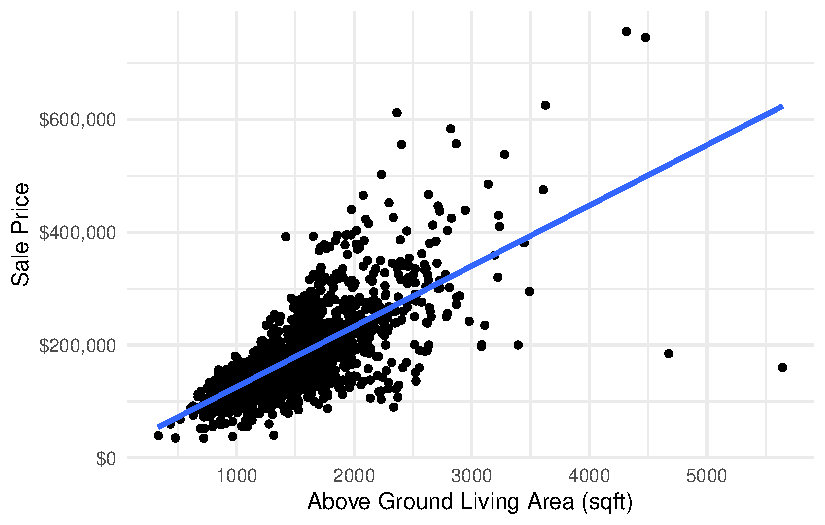
\includegraphics{118_M_SLR_Notes_files/figure-pdf/unnamed-chunk-2-1.pdf}

}

\end{figure}

\hypertarget{correlation}{%
\section{Correlation}\label{correlation}}

Correlation always takes on values between -1 and 1, describes the
strength of the linear relationship between two variables.

\includesvg{118_M_SLR_Notes_files/mediabag/correlation-examples.svg}

\begin{Shaded}
\begin{Highlighting}[]
\FunctionTok{cor}\NormalTok{(housingdata}\SpecialCharTok{$}\NormalTok{GrLivArea, housingdata}\SpecialCharTok{$}\NormalTok{SalePrice)}
\end{Highlighting}
\end{Shaded}

\begin{verbatim}
[1] 0.7086245
\end{verbatim}

\hypertarget{correlation-does-not-imply-causation}{%
\section{Correlation Does Not Imply
Causation}\label{correlation-does-not-imply-causation}}

\includegraphics{https://matt-rickard.ghost.io/content/images/2022/05/image.png}

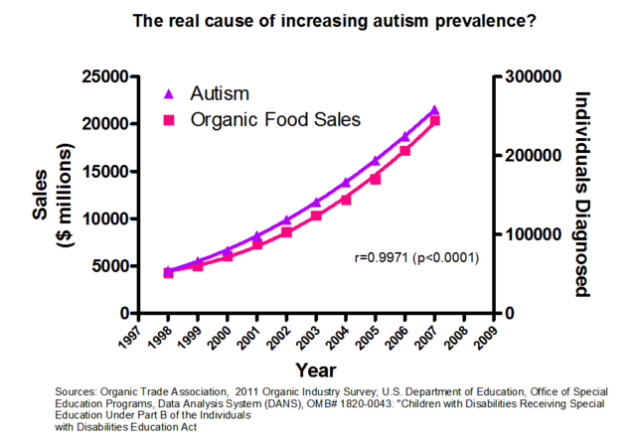
\includegraphics[width=0.5\textwidth,height=\textheight]{118_M_SLR_Notes_files/mediabag/correlation.png}

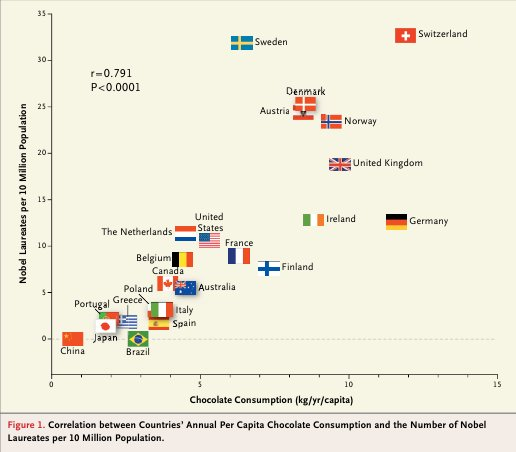
\includegraphics[width=0.5\textwidth,height=\textheight]{118_M_SLR_Notes_files/mediabag/TWQaB.jpg}

\hypertarget{could-be}{%
\subsection{Could be:}\label{could-be}}

\begin{itemize}
\item
  Random coincidence
\item
  Reverse causality
\item
  Confounding variable
\end{itemize}

\hypertarget{equations-and-interpretation-of-coefficients}{%
\section{Equations and Interpretation of
Coefficients}\label{equations-and-interpretation-of-coefficients}}

Want to fit a linear model:

\[
\hat{y} = b_0 + b_1x
\]

To fit a linear regression model we need the \texttt{lm()} function.

\begin{Shaded}
\begin{Highlighting}[]
\CommentTok{\#lm(dependent\_variable \textasciitilde{} independent\_variable, data = dataset)}
\FunctionTok{lm}\NormalTok{(SalePrice }\SpecialCharTok{\textasciitilde{}}\NormalTok{ GrLivArea, }\AttributeTok{data=}\NormalTok{housingdata)}
\end{Highlighting}
\end{Shaded}

\begin{verbatim}

Call:
lm(formula = SalePrice ~ GrLivArea, data = housingdata)

Coefficients:
(Intercept)    GrLivArea  
    18569.0        107.1  
\end{verbatim}

\begin{Shaded}
\begin{Highlighting}[]
\CommentTok{\#OR}

\FunctionTok{lm}\NormalTok{(SalePrice }\SpecialCharTok{\textasciitilde{}}\NormalTok{ GrLivArea, }\AttributeTok{data=}\NormalTok{housingdata) }\SpecialCharTok{\%\textgreater{}\%} 
  \FunctionTok{summary}\NormalTok{()}
\end{Highlighting}
\end{Shaded}

\begin{verbatim}

Call:
lm(formula = SalePrice ~ GrLivArea, data = housingdata)

Residuals:
    Min      1Q  Median      3Q     Max 
-462999  -29800   -1124   21957  339832 

Coefficients:
             Estimate Std. Error t value Pr(>|t|)    
(Intercept) 18569.026   4480.755   4.144 3.61e-05 ***
GrLivArea     107.130      2.794  38.348  < 2e-16 ***
---
Signif. codes:  0 '***' 0.001 '**' 0.01 '*' 0.05 '.' 0.1 ' ' 1

Residual standard error: 56070 on 1458 degrees of freedom
Multiple R-squared:  0.5021,    Adjusted R-squared:  0.5018 
F-statistic:  1471 on 1 and 1458 DF,  p-value: < 2.2e-16
\end{verbatim}

\hypertarget{tidy-it-up-with-broom}{%
\section[Tidy it up with \texttt{broom} ]{\texorpdfstring{Tidy it up
with \texttt{broom}
\protect
\includegraphics[width=0.1\textwidth,height=\textheight]{118_M_SLR_Notes_files/mediabag/logo.png}}{Tidy it up with broom }}\label{tidy-it-up-with-broom}}

\begin{Shaded}
\begin{Highlighting}[]
\FunctionTok{library}\NormalTok{(broom)}
\FunctionTok{library}\NormalTok{(kableExtra)}

\CommentTok{\#prettier}
\FunctionTok{lm}\NormalTok{(SalePrice }\SpecialCharTok{\textasciitilde{}}\NormalTok{ GrLivArea, }\AttributeTok{data=}\NormalTok{housingdata) }\SpecialCharTok{\%\textgreater{}\%} 
  \FunctionTok{tidy}\NormalTok{() }\SpecialCharTok{\%\textgreater{}\%} 
  \FunctionTok{kbl}\NormalTok{() }\SpecialCharTok{\%\textgreater{}\%} 
  \FunctionTok{kable\_styling}\NormalTok{()}
\end{Highlighting}
\end{Shaded}

\begin{table}
\centering
\begin{tabular}[t]{l|r|r|r|r}
\hline
term & estimate & std.error & statistic & p.value\\
\hline
(Intercept) & 18569.0259 & 4480.754549 & 4.144174 & 3.61e-05\\
\hline
GrLivArea & 107.1304 & 2.793621 & 38.348207 & 0.00e+00\\
\hline
\end{tabular}
\end{table}

To interpret the y-intercept coefficient (\(b_0\)):

\begin{itemize}
\tightlist
\item
  When \texttt{x} is 0, we predict \texttt{y} to be \(b_0\).
\item
  In this case, when a house has NO above ground square footage, we
  predict it will cost \$18,569.
\end{itemize}

\begin{tcolorbox}[enhanced jigsaw, colback=white, breakable, colframe=quarto-callout-tip-color-frame, colbacktitle=quarto-callout-tip-color!10!white, left=2mm, toptitle=1mm, opacitybacktitle=0.6, arc=.35mm, rightrule=.15mm, opacityback=0, bottomtitle=1mm, coltitle=black, titlerule=0mm, title=\textcolor{quarto-callout-tip-color}{\faLightbulb}\hspace{0.5em}{Tip}, bottomrule=.15mm, toprule=.15mm, leftrule=.75mm]

Note that the interpretation of the y-intercept doesn't always make
sense.

In this case, what does it mean for a house to have no above ground
square footage? Is it only a basement? Only a plot of land with no
house?

\end{tcolorbox}

To interpret the slope coefficient (\(b_1\)):

\begin{itemize}
\tightlist
\item
  For every 1 unit increase in \texttt{x}, we expect a \(b_1\) unit
  increase in \texttt{y}, on average.
\item
  In this case, for every 1 additional square foot above ground in a
  house, we expect an \$107 increase in the sales price of the house.
\end{itemize}

\hypertarget{assumptions-residuals-and-residual-plots}{%
\section{Assumptions, Residuals, and Residual
Plots}\label{assumptions-residuals-and-residual-plots}}

\hypertarget{assumptions-of-linear-regression}{%
\subsection{Assumptions of Linear
Regression:}\label{assumptions-of-linear-regression}}

\begin{itemize}
\tightlist
\item
  \textbf{Linearity:} The relationship between X and the mean of Y is
  linear -- look at scatterplot
\item
  \textbf{Homoscedasticity:} The variance of residual is the same for
  any value of X -- look at fitted vs.~residuals plot
\item
  \textbf{Independence:} Observations are independent of each other --
  think about context
\item
  \textbf{Normality:} For any fixed value of X, Y is normally
  distributed. -- check the QQ plot
\end{itemize}

\hypertarget{check-the-scatterplot}{%
\subsection{Check the scatterplot}\label{check-the-scatterplot}}

\begin{Shaded}
\begin{Highlighting}[]
\NormalTok{housingdata }\SpecialCharTok{\%\textgreater{}\%} 
  \FunctionTok{ggplot}\NormalTok{(}\FunctionTok{aes}\NormalTok{(}\AttributeTok{x=}\NormalTok{GrLivArea, }\AttributeTok{y=}\NormalTok{SalePrice)) }\SpecialCharTok{+} 
  \FunctionTok{geom\_point}\NormalTok{(}\AttributeTok{pch=}\DecValTok{16}\NormalTok{) }\SpecialCharTok{+} 
  \FunctionTok{geom\_smooth}\NormalTok{(}\AttributeTok{method=}\NormalTok{lm, }\AttributeTok{se=}\ConstantTok{FALSE}\NormalTok{) }\SpecialCharTok{+}
  \FunctionTok{scale\_y\_continuous}\NormalTok{(}\AttributeTok{labels =} \FunctionTok{dollar\_format}\NormalTok{(}\AttributeTok{prefix=}\StringTok{"$"}\NormalTok{)) }\SpecialCharTok{+} 
  \FunctionTok{labs}\NormalTok{(}\AttributeTok{x =} \StringTok{"Above Ground Living Area (sqft)"}\NormalTok{, }\AttributeTok{y =} \StringTok{"Sale Price"}\NormalTok{) }\SpecialCharTok{+} 
  \FunctionTok{theme\_minimal}\NormalTok{()}
\end{Highlighting}
\end{Shaded}

\begin{verbatim}
`geom_smooth()` using formula = 'y ~ x'
\end{verbatim}

\begin{figure}[H]

{\centering 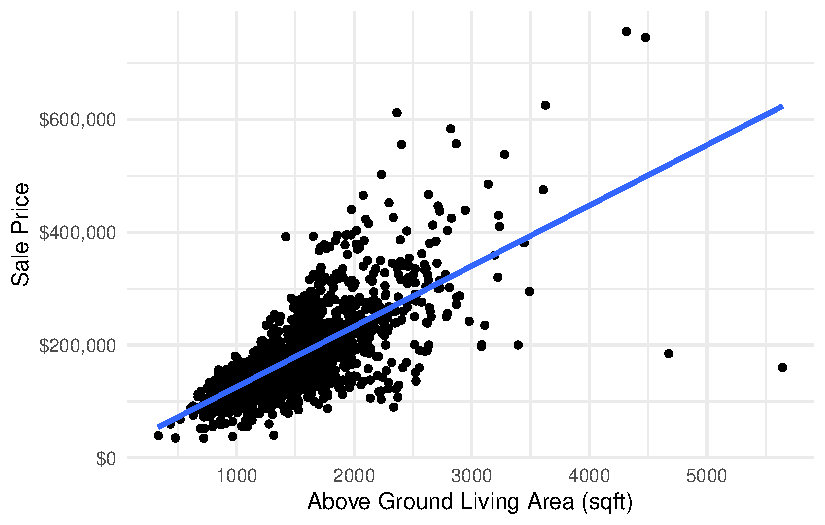
\includegraphics{118_M_SLR_Notes_files/figure-pdf/unnamed-chunk-6-1.pdf}

}

\end{figure}

Some examples of nonlinear plots:

\begin{figure}

{\centering \includegraphics{118_M_SLR_Notes_files/mediabag/scatter-plot-example.png}

}

\caption{Credit: chartio}

\end{figure}

\hypertarget{fitted-vs.-residuals-plot-and-qqplots}{%
\subsection{fitted vs.~residuals plot and
QQplots}\label{fitted-vs.-residuals-plot-and-qqplots}}

\begin{Shaded}
\begin{Highlighting}[]
\CommentTok{\# save our lm() as fit}
\NormalTok{fit }\OtherTok{\textless{}{-}} \FunctionTok{lm}\NormalTok{(SalePrice }\SpecialCharTok{\textasciitilde{}}\NormalTok{ GrLivArea, }\AttributeTok{data=}\NormalTok{housingdata)}
\end{Highlighting}
\end{Shaded}

\begin{Shaded}
\begin{Highlighting}[]
\FunctionTok{library}\NormalTok{(ggfortify)}
\FunctionTok{autoplot}\NormalTok{(fit, }\AttributeTok{which=}\DecValTok{1}\NormalTok{)}
\end{Highlighting}
\end{Shaded}

\begin{figure}[H]

{\centering 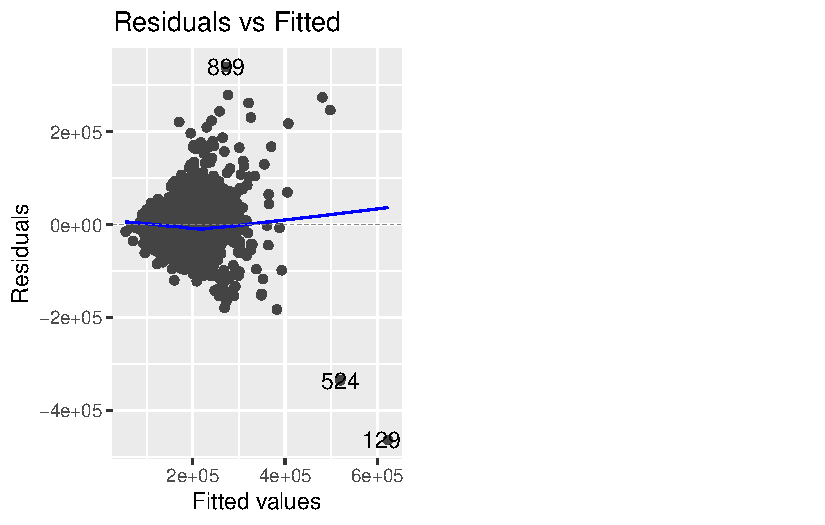
\includegraphics{118_M_SLR_Notes_files/figure-pdf/unnamed-chunk-8-1.pdf}

}

\end{figure}

Some other examples:

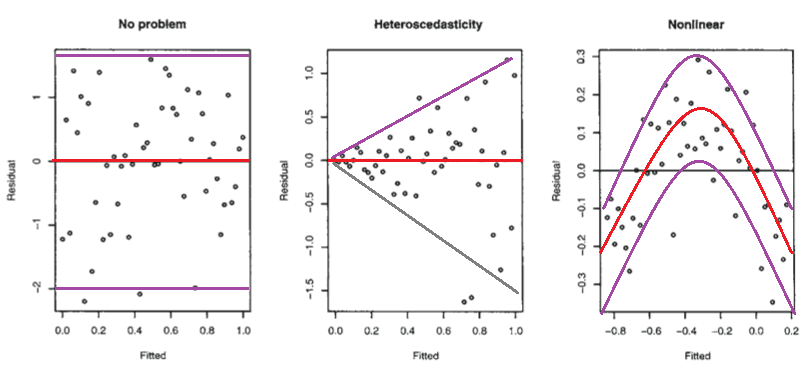
\includegraphics{118_M_SLR_Notes_files/mediabag/RU17l.png}

\hypertarget{qq-plot}{%
\subsection{QQ plot}\label{qq-plot}}

\begin{Shaded}
\begin{Highlighting}[]
\FunctionTok{autoplot}\NormalTok{(fit, }\AttributeTok{which=}\DecValTok{2}\NormalTok{)}
\end{Highlighting}
\end{Shaded}

\begin{figure}[H]

{\centering 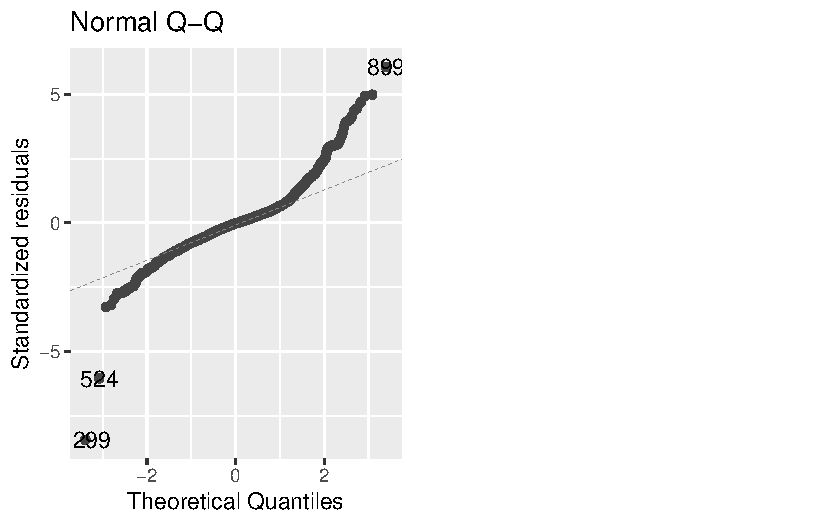
\includegraphics{118_M_SLR_Notes_files/figure-pdf/unnamed-chunk-9-1.pdf}

}

\end{figure}

Some other examples:

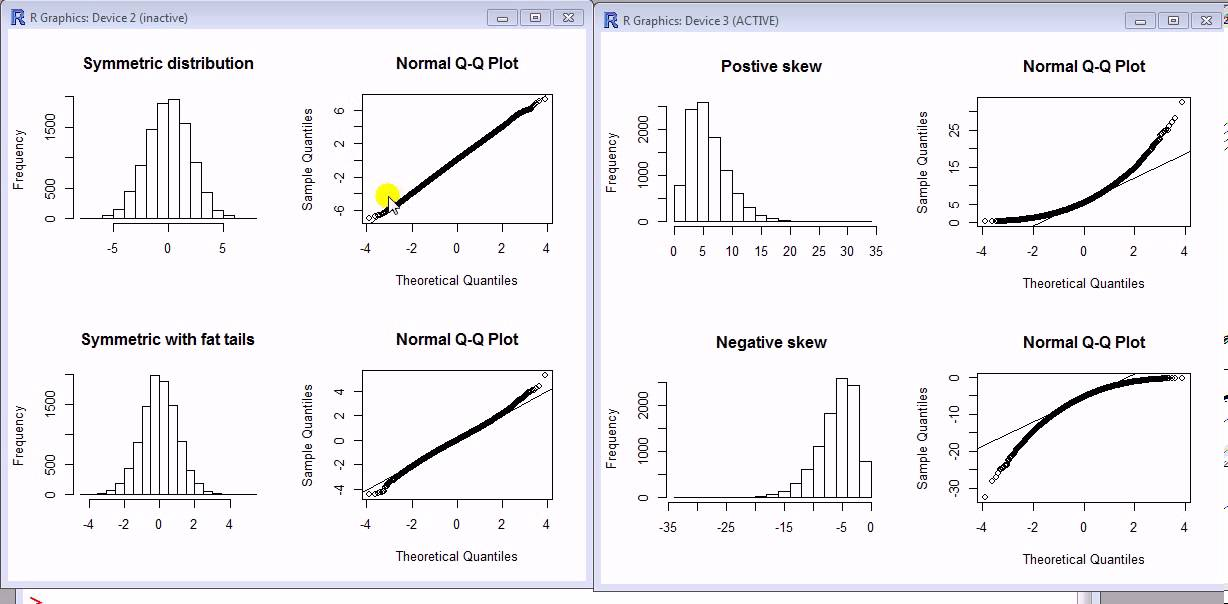
\includegraphics{118_M_SLR_Notes_files/mediabag/maxresdefault.jpg}

\hypertarget{prediction}{%
\section{Prediction}\label{prediction}}

Suppose you are selling your 2000 sqft house. Use the model above to
make a prediction for the

\begin{Shaded}
\begin{Highlighting}[]
\NormalTok{newdata }\OtherTok{\textless{}{-}} \FunctionTok{data.frame}\NormalTok{(}\AttributeTok{GrLivArea =} \FunctionTok{c}\NormalTok{(}\DecValTok{2000}\NormalTok{))}
\FunctionTok{predict}\NormalTok{(fit, newdata)}
\end{Highlighting}
\end{Shaded}

\begin{verbatim}
       1 
232829.7 
\end{verbatim}

\hypertarget{interpolation-vs.-extrapolation}{%
\subsection{Interpolation
vs.~Extrapolation}\label{interpolation-vs.-extrapolation}}

\textbf{Interpolation} is a method of estimating a hypothetical value
that exists within a data set.

\textbf{Extrapolation} is a method of estimation for hypothetical values
that fall outside a data set.

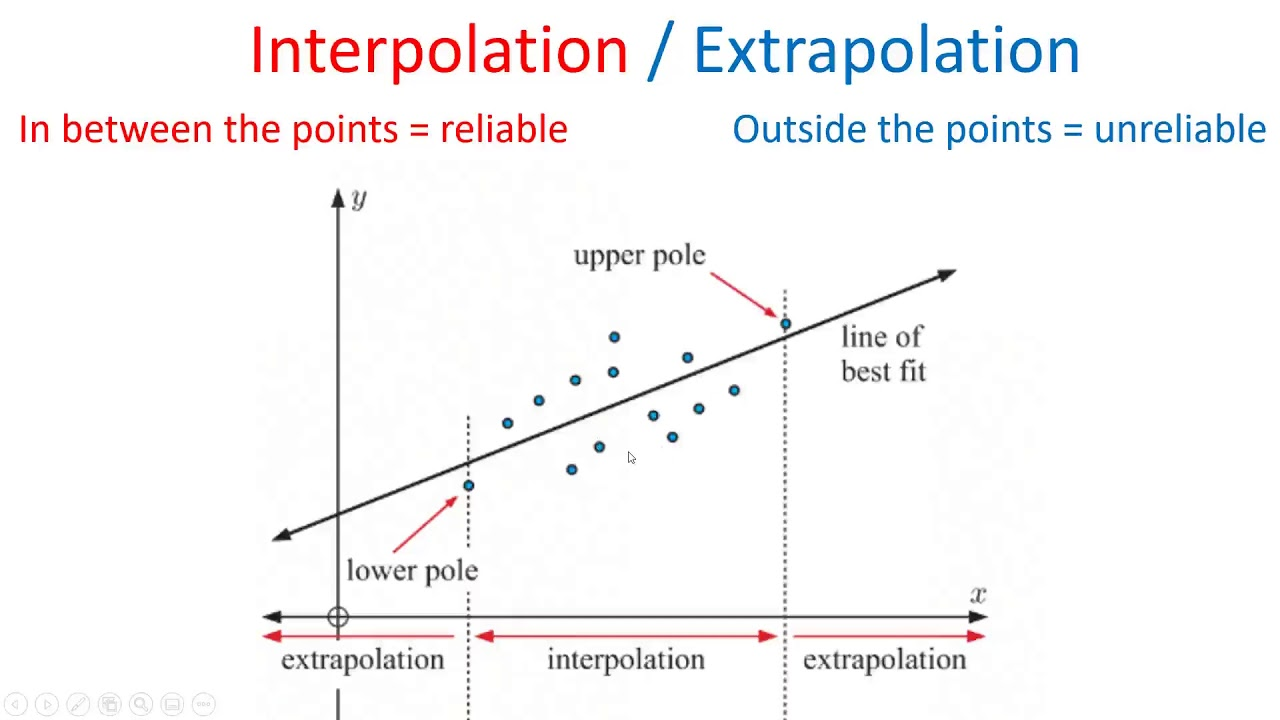
\includegraphics{118_M_SLR_Notes_files/mediabag/maxresdefault1.jpg}



\end{document}
